\documentclass[journal,12pt,twocolumn]{IEEEtran}

\usepackage{setspace}
\usepackage{gensymb}
\singlespacing
\usepackage[cmex10]{amsmath}
\usepackage{multirow}
\usepackage{amsthm}
\usepackage{mathrsfs}
\usepackage{txfonts}
\usepackage{stfloats}
\usepackage{bm}
\usepackage{cite}
\usepackage{cases}
\usepackage{subfig}

\usepackage{longtable}

\usepackage{enumitem}
\usepackage{mathtools}
\usepackage{steinmetz}
\usepackage{tikz}
\usepackage{circuitikz}
\usepackage{verbatim}
\usepackage{tfrupee}
\usepackage[breaklinks=true]{hyperref}
\usepackage{graphicx}
\usepackage{tkz-euclide}

\usetikzlibrary{calc,math}
\usepackage{listings}
    \usepackage{color}                                            %%
    \usepackage{array}                                            %%
    \usepackage{longtable}                                        %%
    \usepackage{calc}                                             %%
    \usepackage{multirow}                                         %%
    \usepackage{hhline}                                           %%
    \usepackage{ifthen}                                           %%
    \usepackage{lscape}     
\usepackage{multicol}
\usepackage{chngcntr}

\DeclareMathOperator*{\Res}{Res}

\renewcommand\thesection{\arabic{section}}
\renewcommand\thesubsection{\thesection.\arabic{subsection}}
\renewcommand\thesubsubsection{\thesubsection.\arabic{subsubsection}}

\renewcommand\thesectiondis{\arabic{section}}
\renewcommand\thesubsectiondis{\thesectiondis.\arabic{subsection}}
\renewcommand\thesubsubsectiondis{\thesubsectiondis.\arabic{subsubsection}}


\hyphenation{op-tical net-works semi-conduc-tor}
\def\inputGnumericTable{}                                 %%

\lstset{
%language=C,
frame=single, 
breaklines=true,
columns=fullflexible
}
\graphicspath{{./Figures/}}
\begin{document}


\newtheorem{theorem}{Theorem}[section]
\newtheorem{problem}{Problem}
\newtheorem{proposition}{Proposition}[section]
\newtheorem{lemma}{Lemma}[section]
\newtheorem{corollary}[theorem]{Corollary}
\newtheorem{example}{Example}[section]
\newtheorem{definition}[problem]{Definition}

\newcommand{\BEQA}{\begin{eqnarray}}
\newcommand{\EEQA}{\end{eqnarray}}
\newcommand{\define}{\stackrel{\triangle}{=}}
\bibliographystyle{IEEEtran}
\raggedbottom
\setlength{\parindent}{0pt}
\providecommand{\mbf}{\mathbf}
\providecommand{\pr}[1]{\ensuremath{\Pr\left(#1\right)}}
\providecommand{\qfunc}[1]{\ensuremath{Q\left(#1\right)}}
\providecommand{\sbrak}[1]{\ensuremath{{}\left[#1\right]}}
\providecommand{\lsbrak}[1]{\ensuremath{{}\left[#1\right.}}
\providecommand{\rsbrak}[1]{\ensuremath{{}\left.#1\right]}}
\providecommand{\brak}[1]{\ensuremath{\left(#1\right)}}
\providecommand{\lbrak}[1]{\ensuremath{\left(#1\right.}}
\providecommand{\rbrak}[1]{\ensuremath{\left.#1\right)}}
\providecommand{\cbrak}[1]{\ensuremath{\left\{#1\right\}}}
\providecommand{\lcbrak}[1]{\ensuremath{\left\{#1\right.}}
\providecommand{\rcbrak}[1]{\ensuremath{\left.#1\right\}}}
\theoremstyle{remark}
\newtheorem{rem}{Remark}
\newcommand{\sgn}{\mathop{\mathrm{sgn}}}
\providecommand{\abs}[1]{\left\vert#1\right\vert}
\providecommand{\res}[1]{\Res\displaylimits_{#1}} 
\providecommand{\norm}[1]{\left\lVert#1\right\rVert}
%\providecommand{\norm}[1]{\lVert#1\rVert}
\providecommand{\mtx}[1]{\mathbf{#1}}
\providecommand{\mean}[1]{E\left[ #1 \right]}
\providecommand{\fourier}{\overset{\mathcal{F}}{ \rightleftharpoons}}
%\providecommand{\hilbert}{\overset{\mathcal{H}}{ \rightleftharpoons}}
\providecommand{\system}{\overset{\mathcal{H}}{ \longleftrightarrow}}
	%\newcommand{\solution}[2]{\textbf{Solution:}{#1}}
\newcommand{\solution}{\noindent \textbf{Solution: }}
\newcommand{\cosec}{\,\text{cosec}\,}
\providecommand{\dec}[2]{\ensuremath{\overset{#1}{\underset{#2}{\gtrless}}}}
\newcommand{\myvec}[1]{\ensuremath{\begin{pmatrix}#1\end{pmatrix}}}
\newcommand{\mydet}[1]{\ensuremath{\begin{vmatrix}#1\end{vmatrix}}}
\newcommand*{\permcomb}[4][0mu]{{{}^{#3}\mkern#1#2_{#4}}}
\newcommand*{\perm}[1][-3mu]{\permcomb[#1]{P}}
\newcommand*{\comb}[1][-1mu]{\permcomb[#1]{C}}
\numberwithin{equation}{subsection}
\makeatletter
\@addtoreset{figure}{problem}
\makeatother
\let\StandardTheFigure\thefigure
\let\vec\mathbf
\renewcommand{\thefigure}{\theproblem}
\def\putbox#1#2#3{\makebox[0in][l]{\makebox[#1][l]{}\raisebox{\baselineskip}[0in][0in]{\raisebox{#2}[0in][0in]{#3}}}}
     \def\rightbox#1{\makebox[0in][r]{#1}}
     \def\centbox#1{\makebox[0in]{#1}}
     \def\topbox#1{\raisebox{-\baselineskip}[0in][0in]{#1}}
     \def\midbox#1{\raisebox{-0.5\baselineskip}[0in][0in]{#1}}
\vspace{3cm}
\title{GATE Assignment 1}
\author{Sujal - AI20BTECH11020}
\maketitle
\newpage
\bigskip
\renewcommand{\thefigure}{\theenumi}
\renewcommand{\thetable}{\theenumi}
Download all latex codes from 

\begin{lstlisting}
https://github.com/https://github.com/sujal100/EE3900/
\end{lstlisting}

\section{Problem}
\textbf{(GATE EC 2015 - Q51)} In the system shown in Figure(a), $m(t)$ is a low-pass signal with bandwidth $W$ Hz. The frequency response of the band-pass filter $H(f)$ is shown in Figure(b). If it is described that the output signal $z(t)=10x(t)$, the maximum value of $W$ (in Hz) should be strictly less than \underline{\hspace{2cm}}
\begin{figure}[!h]
\centering
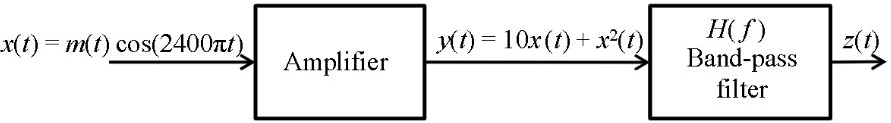
\includegraphics[width=\columnwidth]{question_1.png}
\caption{(a)}
\end{figure}
\begin{figure}[!h]
\centering
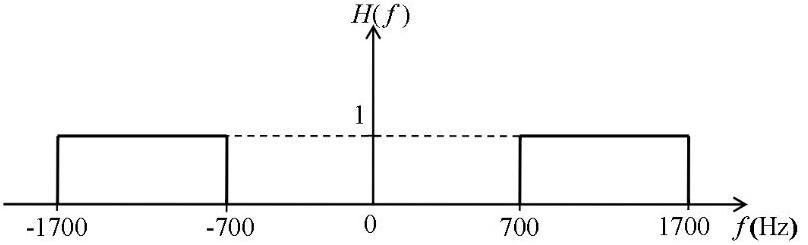
\includegraphics[width=\columnwidth]{question_2.png}
\caption{(b)}
\end{figure}
\section{Solution}
We have the input signal $$x(t)=m(t) \cos (2400 \pi t) = m(t) \cos (\omega t)$$
And, $\omega=2400 \pi$ rad then, $ f = 1200 $ Hz
\begin{align}
y(t) &= 10 x(t)+x^{2}(t)\\
     &= 10 m(t) \cos (2400 \pi t)+m^{2}(t) \cos ^{2}(2400 \pi t) \\
     &= 10 m(t) \cos (\omega t)+ m^{2}(t)\left[\frac{\cos (2 \omega t)+1}{2}\right]\\
     &=\underbrace{\frac{m^{2}(t)}{2}}_{\text {+we frequency }}+\underbrace{10 m(t) \cos (\omega t)}_{[\omega-W, \omega+W]}+\underbrace{\frac{m^{2}(t) \cos (2 \omega t)}{2}}_{[2 \omega-2 W, 2 \omega+2 W]}
\end{align}
If a signal x(t) is multiplied by a sinusoidal signal then the Fourier transform of x(t) gets shifted by the frequency of the sinusoid.\\
\begin{figure}[!h]
\centering
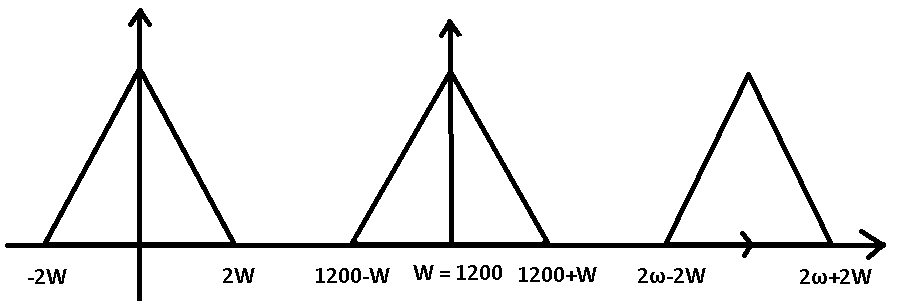
\includegraphics[width=\columnwidth]{sol_1.png}
\caption{Frequency plot}
\end{figure}
So, From the frequency plot, we conclude the following results.
\begin{align}
\text {Results 1 : }&\omega-W>700 \\
& 1200-W>700 \\
& W<500 \\
\text {Results 2 : } &\omega+W<1700 \\
& 1200+W<1700 \\
& W<500 \\
\text {Results 3 : } &\omega -W>2 W \\
& 1200>3 W \\
& W<400 \\
\text {Results 4 : } &2 \omega-2 W>1700 \\
& 2400-1700>2 W \\
& 2 W<700 \\
& W<350
\end{align}
Thus, the above conclusions result in $W < 350$.\\
For $z(t)=10 x(t)$, maximum value of $W$ must be less than $350$ Hz.
\end{document}